\documentclass{article}
%%%%%%%%%%%%%%%%%%%%%%%%%%%%%%%%%%%%%%%%%%%%%%%%%%%%%%%%%%%%%%%%%%%%%%%%%%%%%%%%%%%%%%%%%%%%%%%%%%%%%%%%%%%%%%%%%%%%%%%%%%%%%%%%%%%%%%%%%%%%%%%
\usepackage{generalsnips}
\usepackage{enumitem}
\usepackage{url}
\usepackage{float}
\usepackage{supertabular}
\packagesneeded
\usepackage[top=0.6in, bottom=1in, left=1in, right=1in]{geometry}
\title{Ensayo De Planeación - Empresa hipotética}
\date{2020-Mar-02 22:03:00}
\author{David Gabriel Corzo Mcmath}
%%%%%%%%%%%%%%%%%%%%%%%%%%%%%%%%%%%%%%%%%%%%%%%%%%%%%%%%%%%%%%%%%%%%%%%%%%%%%%%%%%%%%%%%%%%%%%%%%%%%%%%%%%%%%%%%%%%%%%%%%%%%%%%%%%%%%%%%%%%%%%
\begin{document}
\maketitle


%----------------------------------------------------------------------------------------
%%%%%%%%%%%%%%%%%%%%%%%%%%%%%%%%%%%%%%%%%%%%%%%%%%%%%%%%%%%%%%%%%%%%%%%%%%%%%%%%%%%%%%%%%%
%%%%%%%%%%%%%%%%%%%%%%%%%%%%%%%%%%%%%%%%%%%%%%%%%%%%%%%%%%%%%%%%%%%%%%%%%%%%%%%%%%%%%%%%%%
%%%%%%%%%%%%%%%%%%%%%%%%%%%%%%%%%%%%%%%%%%%%%%%%%%%%%%%%%%%%%%%%%%%%%%%%%%%%%%%%%%%%%%%%%%
\section{Empresa hipotética}
La empresa se dedica al desarrollo de software de toda índole. Diseña aplicaciones científicas, educativas y personales es decir que los clientes las mandan a hacer.

%----------------------------------------------------------------------------------------
\subsection{FODA}
\begin{center}
    \begin{tabular}{ | p{8.25cm} | p{8.25cm} | }
         \hline
             \textbf{Fortalezas: } 
             \begin{itemize}
                 \item Tiene autoridades capacitadas con habilidad gerencial 
                 \item Gestiona problemas internos bien 
                 \item Tiene una coordinación interna óptima
             \end{itemize}
             &
             \textbf{Oportunidades: } 
             \begin{itemize}
                 \item Demanda de avances tecnológicos avanzados está en aumento.
                 \item Productos tecnológicos son remunerados muy bien.
             \end{itemize}
             \\ 
         \hline
             \textbf{Debilidades: } 
             \begin{itemize}
                 \item El posicionamiento respecto a las demás empresas es bajo por tener poco tiempo en el mercado.
                 \item La competencia tiende a ganar clientes por el tamaño de la empresa.
             \end{itemize}
             &
             \textbf{Amenazas: } 
             \begin{itemize}
                 \item Los productos del software tienen alta demanda hoy en día.
                 \item Las empresas y los individuos tienen necesidad de tener software fácil de usar y confiables al igual que personalizables.
             \end{itemize}
             \\ 
         \hline
    \end{tabular}
 \end{center}


%----------------------------------------------------------------------------------------
\subsection{Valores}
\begin{itemize}
    \item Nosotros nos complicamos para que usted no.
    \item Privacidad y alta calidad en el trabajo.
    \item Sistema de cyberseguridad altamente confiable.
    \item Soporte técnico con la aplicación.
    \item Aplicaciones altamente confiables que aportan valor en términos de facilidad.
    \item Aplicaciones independientes.
\end{itemize}


%----------------------------------------------------------------------------------------
\subsubsection{Misión y visión}
\begin{itemize}
    \item Misión: ``Crear software y productos que den al cliente poder de utilizarlos con facilidad y que puedan personalizar fácilmente su aplicación''
        \begin{itemize}
            \item ¿Quiénes somos?
                \begin{itemize}
                    \item Somos una empresa que esta comprometida a dar a nuestro clientes los productos con calidad y atención, empleando prácticas de comunicación para entender qué es lo que el cliente quiere exactamente y así poder acertar con más precisión lo que el cliente se imagina. 
                \end{itemize}
                
            \item ¿Cuál es la promesa de servicio?
                \begin{itemize}
                    \item Pretendemos poner a prueba la premisa que el precio de la facilidad de uso de un programa es la falta de personalización del programa.
                \end{itemize}
                
            \item ¿Qué ofrecemos que nos hace únicos?
                \begin{itemize}
                    \item Facilidad y personalización.
                \end{itemize}
                
            \item ¿Quiénes son nuestros clientes?
                \begin{itemize}
                    \item Las personas que estén interesadas en tener aplicaciones que estén altamente mantenidas y que sean versátiles y personalizables.
                \end{itemize}
        \end{itemize}
    
    \item Visión: ``Llegar a ser líder en software por especializarnos en programas fáciles de usar y personalizables''
        \begin{itemize}
            \item \pregunta{Hacia dónde vamos} 
                \begin{itemize}
                    \item Mediante el enfoque que le damos a la facilidad y a la personalización queremos crear algún día aplicaciones altamente funcionales, tan personalizables que no requieran casi nada de mantenimiento. 
                \end{itemize}
                
            \item \pregunta{En qué queremos ser un referente} 
                \begin{itemize}
                    \item Innovadores y excelentes oyentes a lo que nuestros clientes quieren.
                \end{itemize}
                
            \item \pregunta{Cómo nos vemos en el futuro} 
                \begin{itemize}
                    \item Haciendo grandes proyectos para grandes clientes.
                \end{itemize}
                
            \item \pregunta{Cuál será nuestro legado} 
                \begin{itemize}
                    \item La corriente de pensamiento que poder tener una aplicación fácil de usar y personalizable no son mútuamente excluyentes.
                \end{itemize}
        \end{itemize}
\end{itemize}


%----------------------------------------------------------------------------------------
\subsection{Estrategia global de competencia}
\begin{itemize}
    \item La estrategia global de competencia para esta empresa será idealmente la de enfoque ya que se concentra mucho en gente con demandas muy peculiares y a gente con necesidades muy especializadas, una persona común y corriente no demandará que le hagan un app con tantas especificaciones.
    \item La estrategia de producto será especializada, los precios serán por su mayoría acordados exclusivamente con el cliente, además se observa que el mercadeo será sólo hacia un segmento de mercado. 
    \item Los puntos de ventas serán pocos y se darán por su mayoría interacciones virtuales con el cliente.
    \item La estrategia global de competencia.
    \item Se intentará ser una empresa que tenga atención personalizada con el cliente para entender a profundidad qué es lo que necesita.
\end{itemize}


%----------------------------------------------------------------------------------------
\section{Plazos de la planeación estratégica}
\begin{center}
    \begin{supertabular}{ |p{2cm}|p{2cm}|p{5cm}|p{5cm}| }
        \hline
            Plazo & Criterios & Justificación del plazo & Objetivos globales\\
        \hline
            Corto plazo (1 año): 
            & 
            Periodo de recuperación de inversión
            & 
            Dado a que el producto será caro y será una inversión de gran escala dependiendo de las ventas de cada periodo vale la pena planear el posible evento que no se llegue al equilibrio.
            & 
            Dado a que la empresa está en fases iniciales se necesita recuperar el capital para poder llegar a sobrevivir por ahora. Objetivo recuperar un 30\% de utilidades derivadas de las ventas para un lapso de un años.
            \\ 
        \hline
            Mediano Plazo (5 años):
            & 
            Velocidad de cambio en la tecnología.
            & 
            El hecho que la tecnología siempre está cambiando es algo que se tiene que tomar muy en cuenta, por ejemplo si Apple lanza un nuevo teléfono las aplicaciones y el software se tiene que adaptar a los cambios en el sistema operativo de ellos.
            & 
            Dado a que el ambiente tecnológico es uno de los más cambiantes del mercado se tiene que mantener al tanto de qué tanto cambian, esto está alineado al objetivo de Soporte técnico de nuestros productos y también alineado al sistema de seguridad Cybernética. Objetivo: estar el tanto de los cambios y surgimientos de nuevas tecnologías en un lapso de 5 años.
            \\ 
        \hline
            Largo plazo (10 años): 
            & 
            Barreras de entrada a nuevos mercados.
            & 
            Conforme vamos creciendo valdría la pena planear el evento de entrar a nuevos mercados a brindar nuestros productos y servicios puede complicarse por las barreras de entrada. 
            & 
            Conforme se expande la red de operación de una empresa se expande se puede llegar a volver un obstáculo entrar a nuevos mercados, alineado con el objetivo de crecer y expandirse. Objetivos: Expandir la red de operación a Centro América y así poder derivar más ganancias, crecer en tamaño de la empresa, ser un potencial líder del mercado para el 2030.
            \\ 
        \multicolumn{4}{|c|}{\tabletail{\hline}}  \\
    \end{supertabular}
\end{center}


%%%%%%%%%%%%%%%%%%%%%%%%%%%%%%%%%%%%%%%%%%%%%%%%%%%%%%%%%%%%%%%%%%%%%%%%%%%%%%%%%%%%%%%%%%
\section{Fuerzas competitivas de Michael Porter}
Debido a que esta empresa es nueva en el mercado, lo que determina la competitividad en estos mercados con más relevancia son los clientes y la competencia.




%----------------------------------------------------------------------------------------
\subsection{Clientes}
Se tiene que tener un conocimiento vasto de quién es mi mercado, mi mercado idealmente son todas las personas que requieran servicios de software a precio diferenciado y por enfoque dado a que son productos especializados en los que se aprecian ciertas características muy rebuscadas como la personalización de un software. Entonces nuestros clientes son todas las personas interesadas en tener software personalizable y fácil de usar. El tamaño del mercado en este sentido sería algo limitado, además no somos los únicos en el mercado que ofrecerá este tipo de productos, los clientes tienen que tomar una decisión acercad de a quién le comprarán.


%----------------------------------------------------------------------------------------
\subsubsection{Competencia en el mercado}
Actualmente los ``tech giants'' son una gran amenaza, pero precisamente por que ellos hacen software restrictivo en cierto sentido, se entiende que los productos que ellos harán serán orientados a la producción en masas, por ende nos diferenciamos, nosotros haríamos software orientado a la persona individual y adaptado a las necesidades puntuales de nuestros clientes. En este aspecto la competencia son las empresas de freelancing, superar a estas empresas probará a ser una labor complicada dado a que ellos se diferencian por su bajo costo. 


\subsection{Conclusión}
Dado a que los competidores son menores y los clientes son limitados se concluye que es un mercado poco competitivo dado a que los factores que determinan la competitividad han salido bajos. La competencia es relativamente baja pero con el reto de también del tamaño del mercado ser pequeño.

%----------------------------------------------------------------------------------------
\subsection{Matriz de posicionamiento}
\begin{figure}[H]
    \centering
    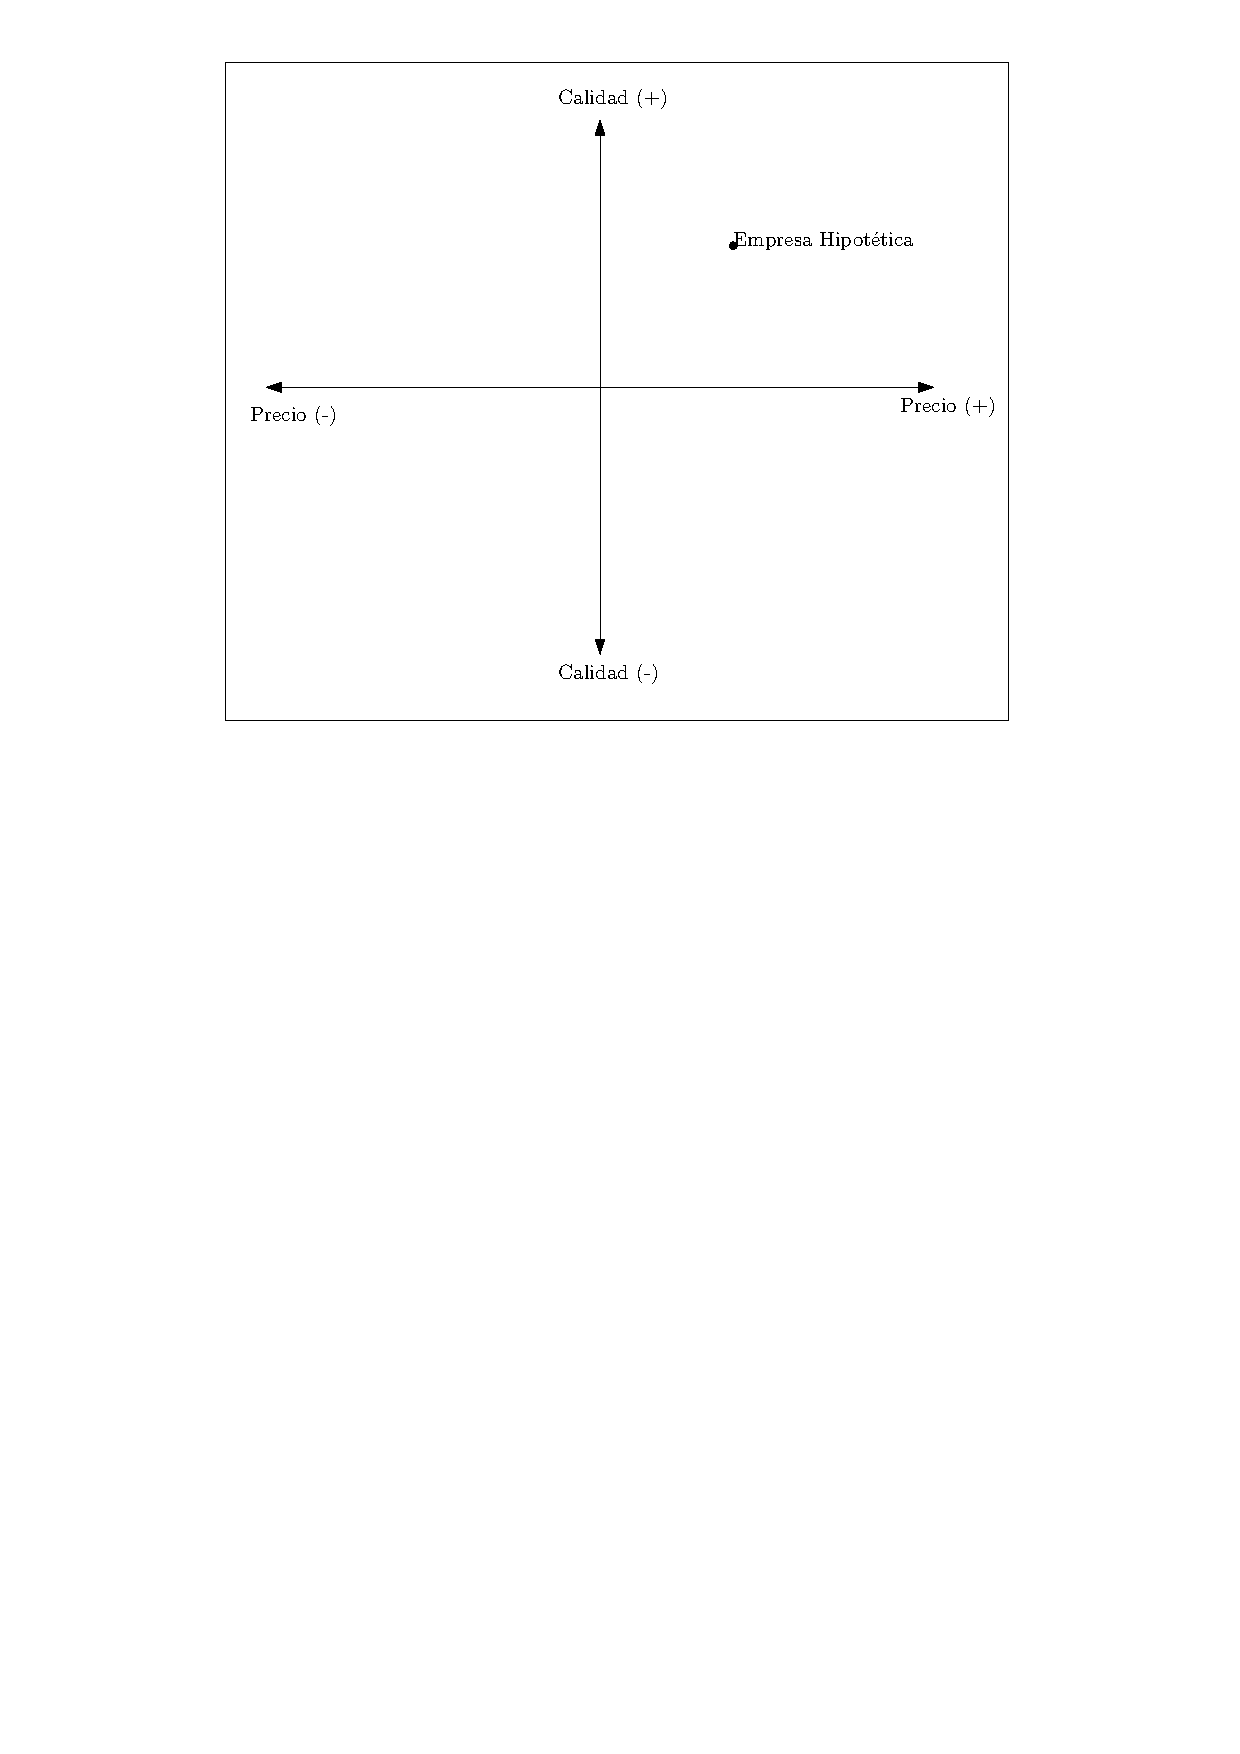
\includegraphics[]{figs/MatrixHipo} 
\end{figure}



%%%%%%%%%%%%%%%%%%%%%%%%%%%%%%%%%%%%%%%%%%%%%%%%%%%%%%%%%%%%%%%%%%%%%%%%%%%%%%%%%%%%%%%%%%
\section{Áreas clave}
\begin{center}
    \begin{supertabular}{ |p{2cm}|p{2cm}|p{5cm}|p{5cm}| }
        \hline
            Áreas clave & Core / Soporte & Descripción y justificación & Alineación con objetivos globales \\
        \hline
            Software de calidad y fácil de usar & 
            Core & 
            Debido a los valores que se han determinado a partir de las tendencias y necesidades de los clientes es necesario que el producto cumpla con las características ofrecidas. & 
            \textbf{Análisis:} Alineado con el objetivo de crear productos fáciles de usar, alineado con la misión. Poder verificar estos objetivos por medio de las ventas, encuestar a los clientes para medir su nivel de satisfacción con el producto. Alinear lo ofrecido con lo entregado al cliente. \textbf{Objetivo global:} Considerar este objetivo para cumplimiento a corto plazo es decir en un lapso de un mes tras haber entregado el primer producto, o en abril de este año. \\ 
        \hline
            Software personalizable & 
            Core & 
            Análisis: Una de las características ofrecidas ha sido precisamente poder personalizar software fácil de usar. & 
            \textbf{Análisis:} Es necesario cumplir con lo que ofrecemos para poder cumplir con el objetivo de expandirnos y quedar bien con nuestros clientes. \textbf{Objetivo global:} Como objetivo tenemos para al largo plazo que la empresa crezca de un 30\% a un 50\% en un lapso de 10 años o en el 2030. \\ 
        \hline
            Atención al cliente & 
            Soporte & 
            Análisis: Parte de lo que implica saber definir qué quiere el cliente es darle mucha atención y asesoramiento, es por eso que es necesario poder darle atención al cliente cuando lo necesite. & 
            \textbf{Análisis:} Para poder posicionarnos mejor es bueno tener una reputación en la que se favorece el trato personal de las gestiones individuales de los clientes. \textbf{Objetivo global:} Para aplicación inmediata a priori de elaborar el primer producto se debe tomar en cuenta que el servicio cumpla con la característica ofrecida, esto se pondrá en práctica desde el primer momento en el cual la empresa esté operando.  \\ 
        \hline
            Software independiente & 
            Soporte & 
            Parte de los que se ofrece es la característica de tener software que no dependa de otros o cuyos procesos internos necesiten configuraciones avanzadas para poder operar, pretendemos evitar que el cliente se encuentre en estas situaciones, por eso es importante que se piense el software con esta característica desde un principio & 
            \textbf{Análisis:} Alineado con el objetivo de cumplir promesas de nuestros servicios. \textbf{Objetivo global:} esta característica debe de ser cumplida desde el momento en el que se empiece la elaboración del primer producto es decir en 1 mes o en abril del presente año. \\ 
        \hline
            Red de distribución & 
            Core & 
            Expandirse ha sido un objetivo de la empresa desde el principio, conforme crezcamos se necesita priorizar la red de distribución.  & 
            \textbf{Análisis:} Alineado con la visión de la empresa. \textbf{Objetivo global:} Para largo plazo (en 10 años o en el 2030) expandir nuestras operaciones a toda Centro América tras haber crecido por lo menos un 50\%. \\ 
        \hline 
            Gestión rápida de problemas & 
            Core & 
            El mantenimiento y soporte técnico de nuestras aplicaciones es una característica principal de nuestros servicios y productos, es por eso que es de vital importancia que se tenga una forma de poder asesorar al cliente si llegase a darse un determinado problema. & 
            \textbf{Análisis:} Alineado con el objetivo de soporte técnico y mantenimiento de nuestros productos, alineado también con el objetivo de responsabilizarnos por nuestros productos. \textbf{Objetivo global:} Este servicio se debe de ofrecer inmediatamente tras haber entregado el primer producto, se estima que en 1 mes o en abril de este año. \\ 
        \hline
    \end{supertabular}
\end{center}


\section{Fuentes}
\begin{enumerate}
    \item \url{https://venturebeat.com/2019/12/30/10-technology-trends-that-will-impact-our-lives-in-2020/}
\end{enumerate}



%%%%%%%%%%%%%%%%%%%%%%%%%%%%%%%%%%%%%%%%%%%%%%%%%%%%%%%%%%%%%%%%%%%%%%%%%%%%%%%%%%%%%%%%%%
\clearpage
\begin{center}
    \thispagestyle{fancy}
    \vspace*{\fill}
    \Huge{\textbf{Constancia de entregas}}
    \vspace*{\fill}
\end{center}
\clearpage

{
    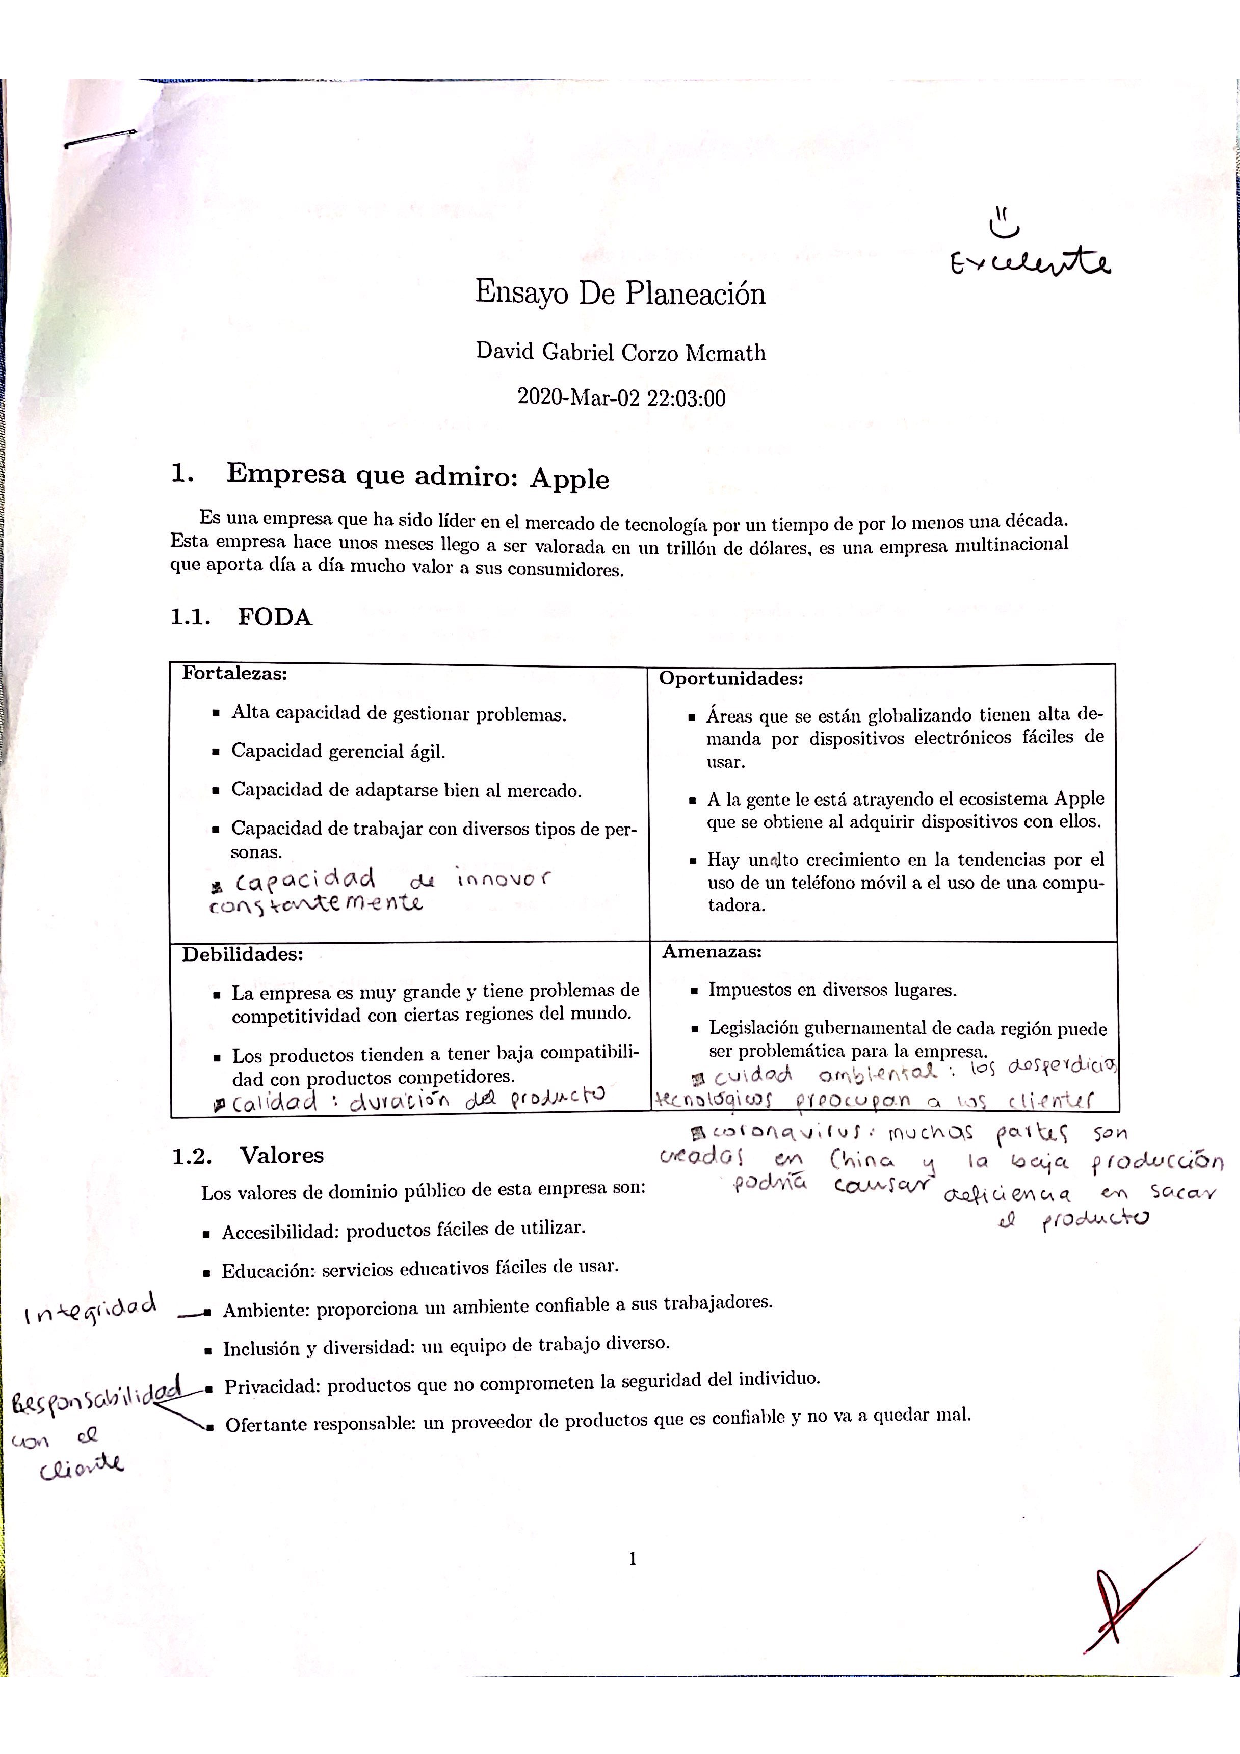
\includepdf[pages=1,pagecommand={\thispagestyle{empty}\section*{\Huge{Primera Entrega}}}]{./entregas/constancia_entregas_completas_1.pdf}
    \includepdf[pages={2-last},pagecommand={\thispagestyle{plain}}]{./entregas/constancia_entregas_completas_1.pdf}
}

{
    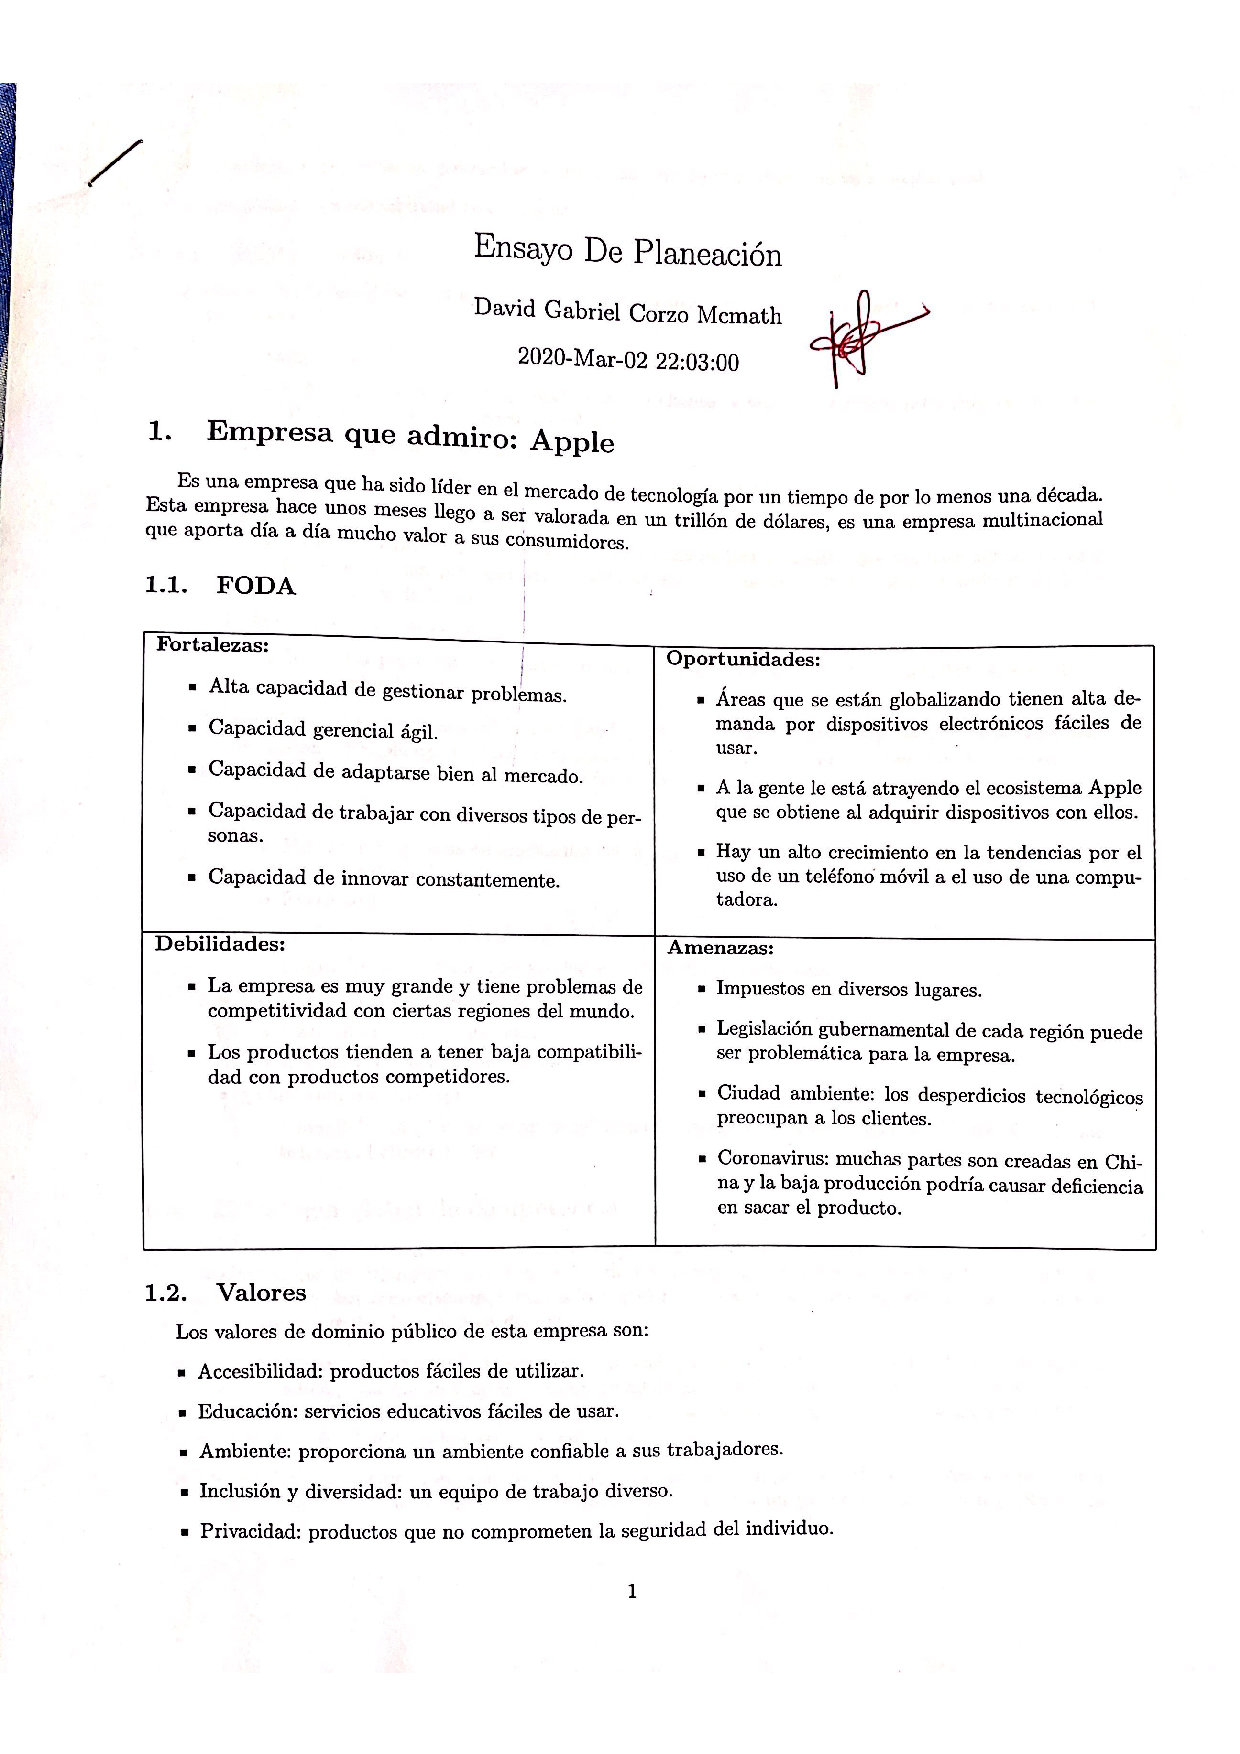
\includepdf[pages=1,pagecommand={\thispagestyle{empty}\section*{\Huge{Segunda entrega}}}]{./entregas/constancia_entregas_completas_2.pdf}
    \includepdf[pages={2-last},pagecommand={\thispagestyle{empty}}]{./entregas/constancia_entregas_completas_2.pdf}
}

{
    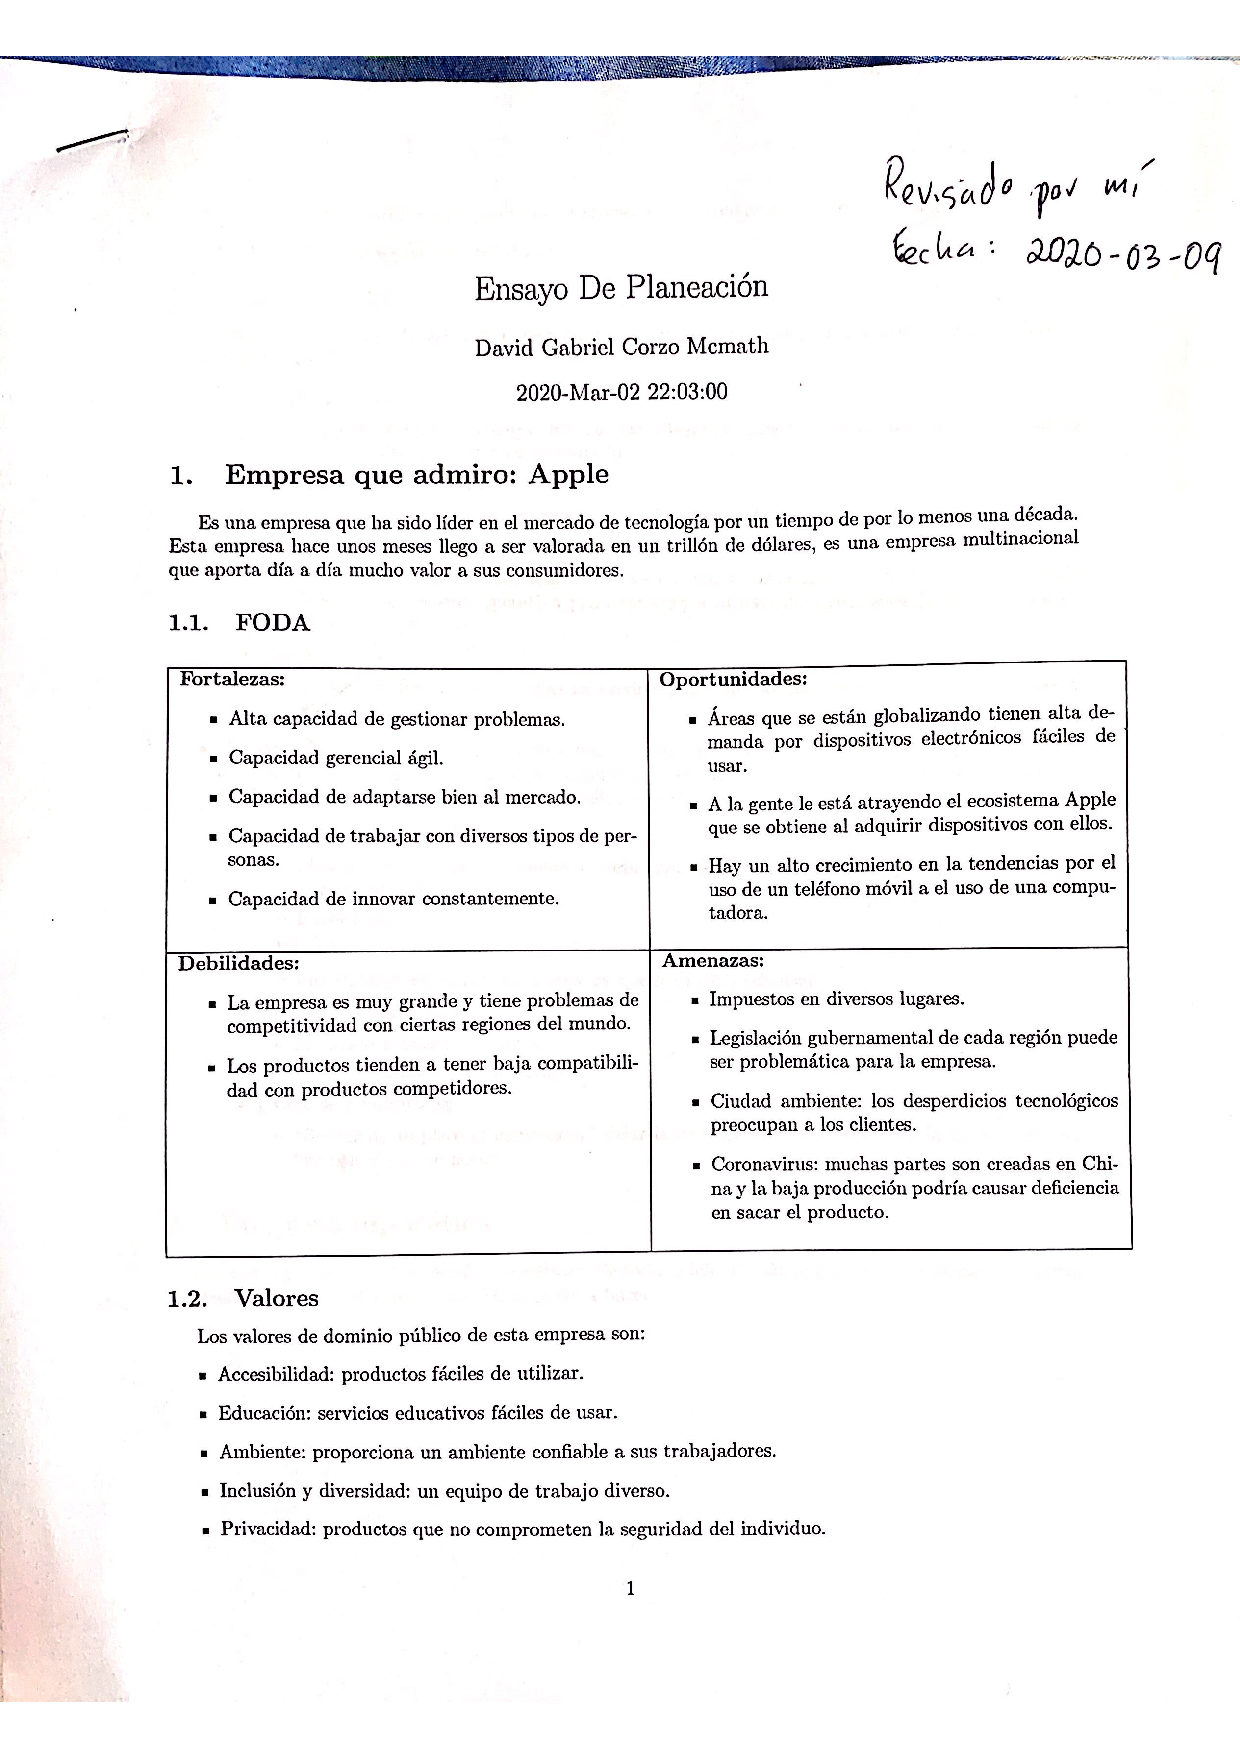
\includepdf[pages=1,pagecommand={\thispagestyle{empty}\section*{\Huge{Tercera Entrega}}}]{./entregas/constancia_entregas_completas_3.pdf}
    \includepdf[pages={2-last},pagecommand={\thispagestyle{empty}}]{./entregas/constancia_entregas_completas_3.pdf}
}

\end{document}


